% ==================================================
\chapter{Results}\label{chap:Results}
% ==================================================

% --------------------------
\section{User Feedback - Usability Study}
% --------------------------



A total of 15 participants from various disciplines including Natural Sciences, Social Sciences, Life Sciences and Computer Science evaluated Scholar Plot. We asked each participant to review the interface and then complete an online survey. Special care was taken to ensure that the participants had correct understanding about the visualization component before they began rating. The participants answered the questions on a Likert scale from 1 to 5 with 1 being strongly disagree and 5 being strongly agree.

Figure \ref{fig:UserStudy} illustrates the mean evaluation for each visualization component. Accuracy, Usability and understandability of Scholar Plot scored the highest $(\mu = 4.2)$ as it is very intuitive and can be used with minimal assistance. Many participants gave us feedback that they mostly liked the visual scheme of Scholar Plot. Another observation is that the participants agree to use Scholar Plot to evaluate themselves $(\mu = 4.1)$. They suggested that Scholar Plot can be improved by adding more funding agencies. Overall, this evaluation indicated that Scholar Plot is a user-friendly tool that complements the CV which can be used to review a scholar's accomplishments. The survey has been approved by the University of Houston Institutional Review Board (IRB).

 \begin{figure}[!htb]
  \centering
  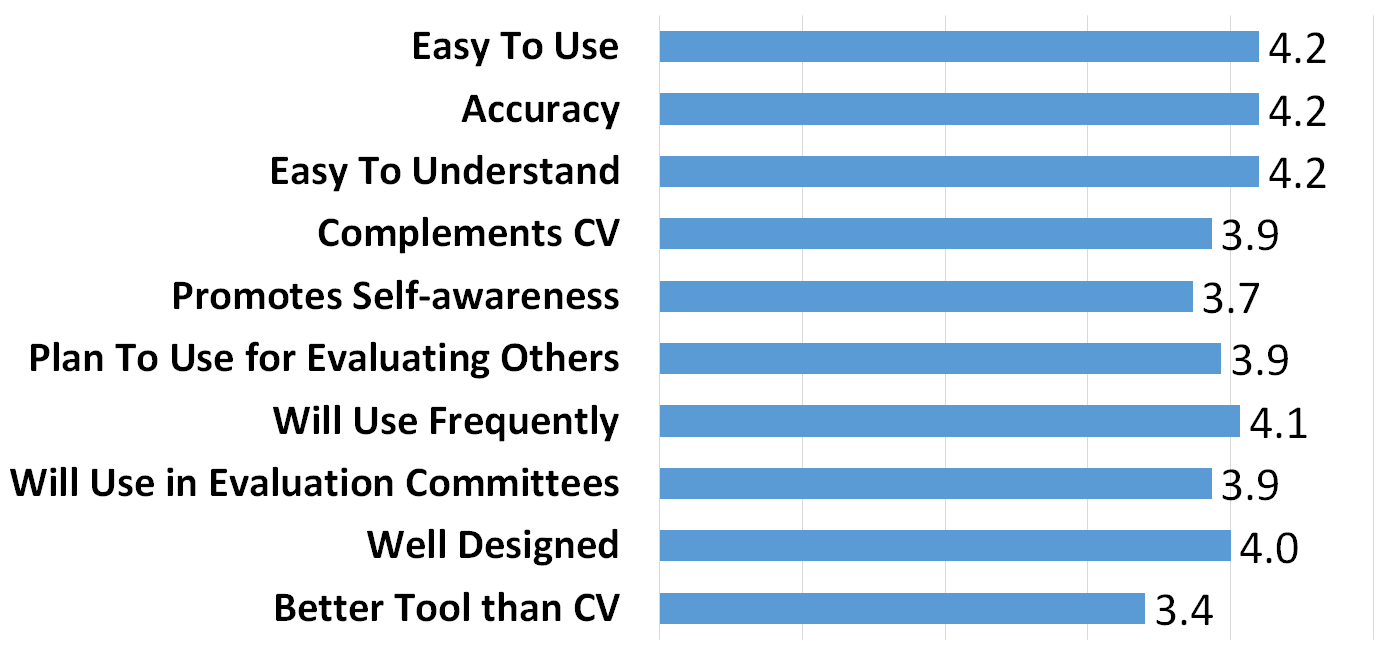
\includegraphics[width=\textwidth]{figures/fig_survey_chart}
%  \vspace{-3ex}
  \caption{Mean evaluation of Scholar Plot. A total of $n=15$ participants evaluated the survey.}
  \label{fig:UserStudy}
\end{figure}



% --------------------------
\section{User Feedback - Focus Group}
% --------------------------

We ran a focus group with 10  Principal Investigators and their post docs at Northwestern University. The participant set included biologists, physicists, computer scientists, and social scientists.  The focus group's suggestions are synopsized as follows:
\begin{description}
\item [Interface team science information.] Participants wanted to see the number and intensity of collaborations for the depicted scholar.
\item [Summarize highly cited papers.] Participants wanted to see explicitly in a side panel the scholar's most popular papers.
\item [Interface journal profile.] Participants wanted to see the specific journals where the scholar publishes most often and their impact factors.
\end{description}

The participants believed that accessorizing the central publication graph with this additional information would support deeper instant comprehension without compromising the elegance of SP's compact visual representation. Specifically, this additional interface would reveal the collaborative nature of the scholar's work, give hints if s/he is regular in specific disciplinary journals or if s/he publishes in a variety of journals (interdisciplinarity), and give the rank of these journals. All this information can also be gleaned by rolling the mouse over the publication graph, reading the tooltips; summarizing it in panels under the graph, however, renders such manual investigation unnecessary.

\begin{figure}[H]
    \centering
    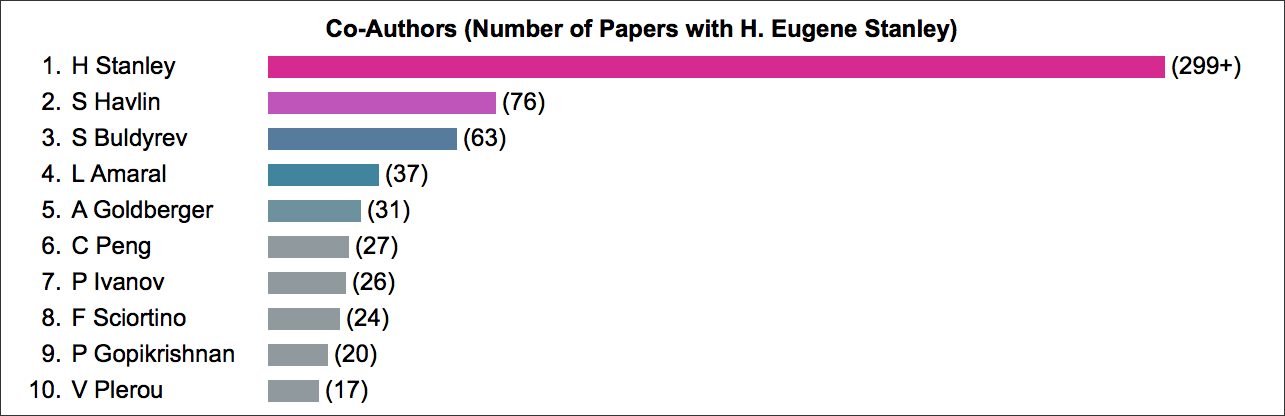
\includegraphics[width=\textwidth]{figures/fig_panel1-N}
    \caption{Panel listing the top collaborators with the selected scholar ranked by the count of the number of publications collaborated.}
    \label{fig:panel1}
\end{figure}

\begin{figure}[H]
    \centering
    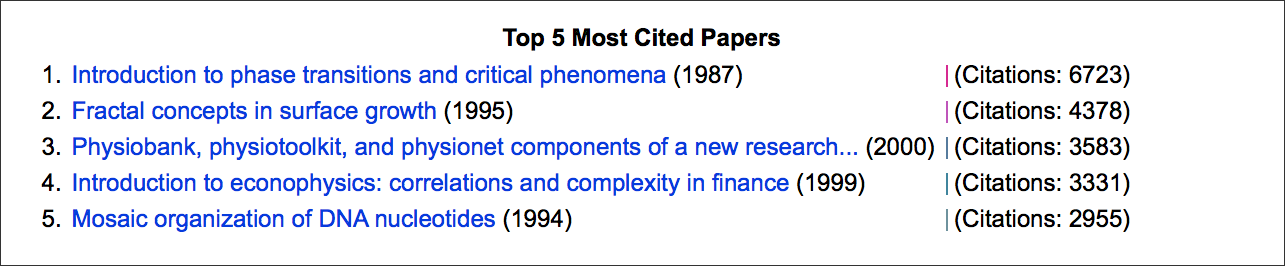
\includegraphics[width=\textwidth]{figures/fig_panel3-N}
    \caption{Panel highlighting the top 5 cited papers of the selected scholar.}
    \label{fig:panel3}
\end{figure}

\begin{figure}[H]
    \centering
    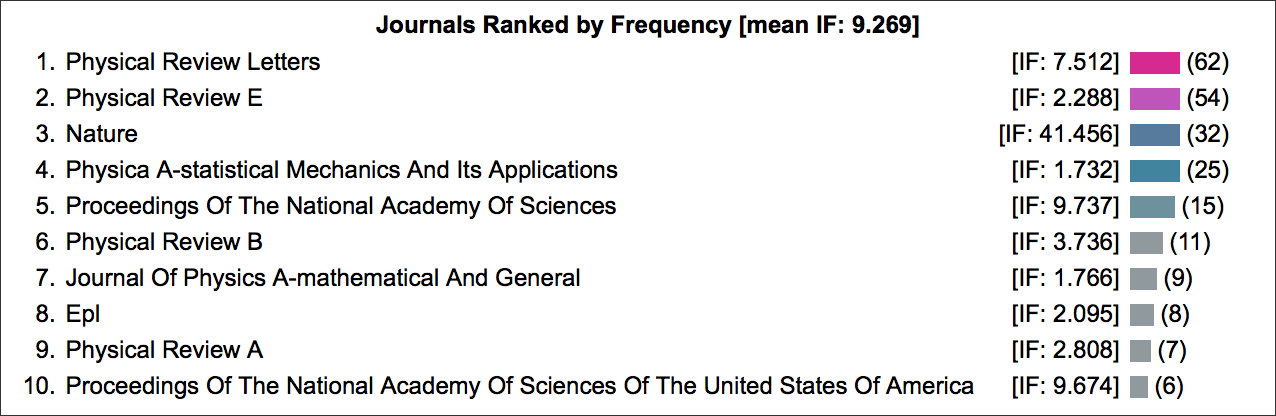
\includegraphics[width=\textwidth]{figures/fig_panel2-N}
    \caption{Panel displaying the top journals ranked by the frequency of publication.}
    \label{fig:panel2}
\end{figure}

\begin{figure}[H]
    \centering
    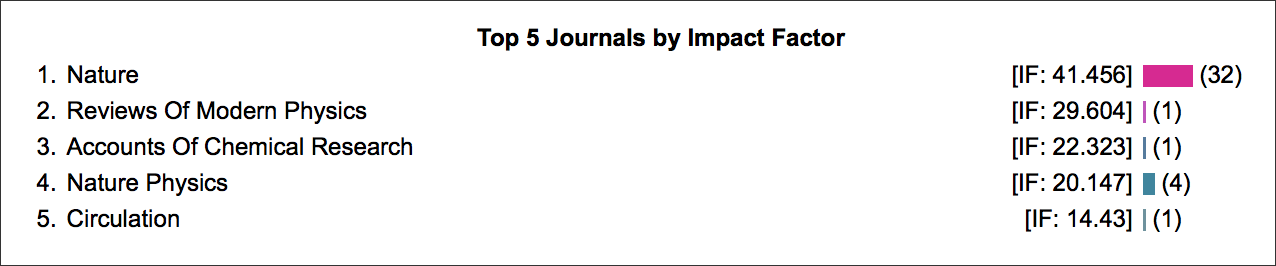
\includegraphics[width=\textwidth]{figures/fig_panel4-N}
    \caption{Panel showing the top 5 journals where the selected scholar published ranked by the impact factor.}
    \label{fig:panel4}
\end{figure}






% --------------------------
\section{Data Analysis}
% --------------------------
For validation of the design choices of academic garden, I used chaired faculty as the ground truth units of analysis. Chaired faculty are well  I run linear models in R to understand the behavior of data. To do this so, the chaired faculty is used as a standard of academic fields. 

The data has been collected in July 2016. This included total 14 different universities . The data collected consists of professors from Computer Science $( n = 248 )$ and Biology $( n = 152 )$ in top 10 schools in the respective fields. The data of chaired faculty collected consists of chaired professors from Computer Science $( n = 61 )$ and Biology $( n = 32 )$ in top 10 schools in the respective fields.


% For tables use
\begin{table*}
\centering
% table caption is above the table
\caption{The list of institutes in Computer Science by rank sourced from U.S. News \cite{usnews}.}
\label{tab:1}       % Give a unique label
% For LaTeX tables use
\begin{tabular}{rl}
\hline\noalign{\smallskip}
Rank & Department of Computer Science \\
\noalign{\smallskip}\hline\noalign{\smallskip}
1 & University of California, Berkeley \\
1 & Carnegie Mellon University \\
1 & Massachusetts Institute of Technology \\
1 & Stanford University \\
5 & University of Illinois at Urbana-Champaign \\
6 & Cornell University \\
6 & University of Washington \\
8 & Princeton University \\
9 & Georgia Institute of Technology \\
10 & University of Texas, Austin  \\
\noalign{\smallskip}\hline
\end{tabular}
\end{table*}



% For tables use
\begin{table*}
\centering
% table caption is above the table
\caption{The list of institutes in Biology by rank sourced from U.S. News \cite{usnews}.}
\label{tab:}       % Give a unique label
% For LaTeX tables use
\begin{tabular}{rl}
\hline\noalign{\smallskip}
Rank & Department of Biology  \\
\noalign{\smallskip}\hline\noalign{\smallskip}
1 & Harvard University \\
1 & Massachusetts Institute of Technology \\
1 & Stanford University \\
4 & University of California, Berkeley \\
5 & California Institute of Technology \\
5 & Johns Hopkins University \\
7 & University of California San Francisco \\
7 & Yale University \\
9 & Princeton University \\
10 & Cornell University \\

\noalign{\smallskip}\hline
\end{tabular}
\end{table*}


The faculty is in the top quartile for either of the 3 criteria (citation, impact factor, and funding), the faculty is the chaired professor, however, the faculty is not in the top quartile for all the 3 criteria, s/he is not a chaired because it is widely considered in academic fields. In computer science, its results of `At Least 1 Top Local Quartile` is significant ( p $<$ 0.05 ) and the real values is shown in Figures \ref{fig:CS-Local-Quartile}. In this model, quartiles are calculated with respect to the department to which the faculty belongs to.

 \begin{figure}
  \centering
  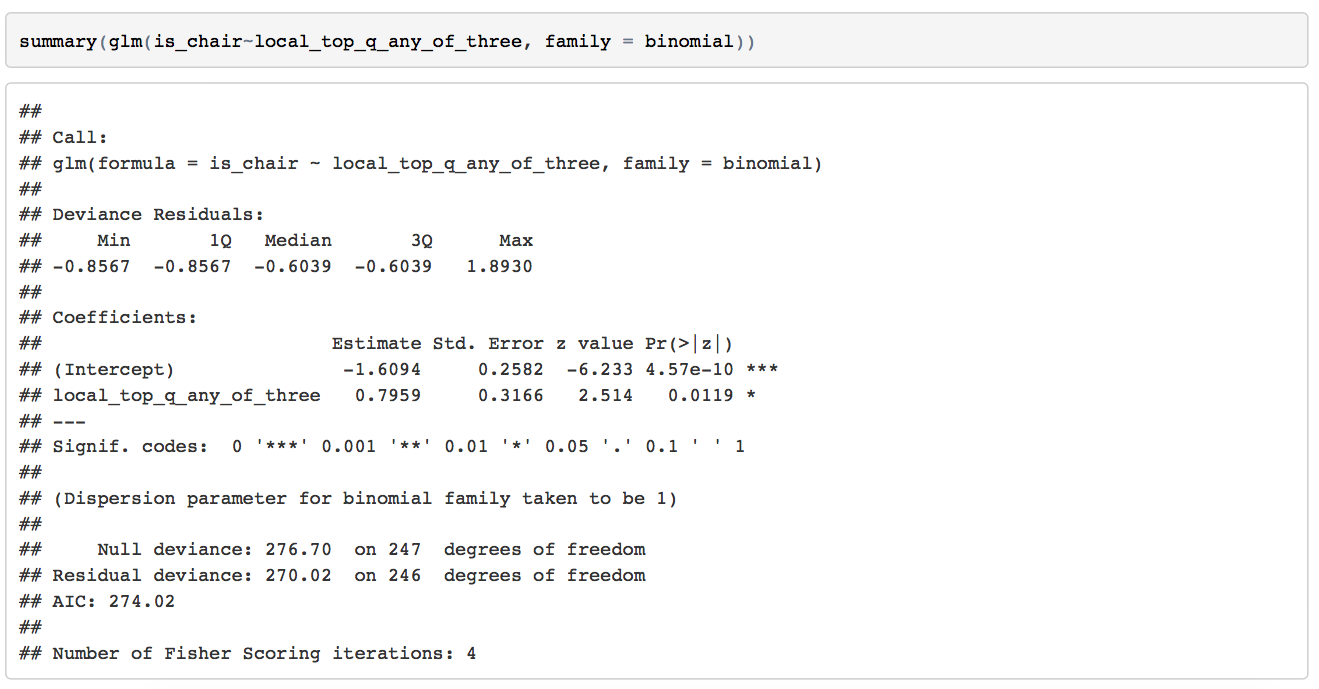
\includegraphics[width=\textwidth]{figures/CS-Local-Quartile}
%  \vspace{-3ex}
  \caption{Screenshot of a result of Linear Model in R}
  \label{fig:CS-Local-Quartile}
\end{figure}

All three criteria are separately factors. In computer science, the significance level in citation is very high ( p $<$ 0.001 ) while impact factor are not significant because computer science faculty does not publish so much journals during their academic years. Also, the funding is also not significant because our funding sources are not included everything which computer science faculty received funding from for example DoD (United States Department of Defense) and DHS (United States Department of Homeland Security).

However, the results are quite different in Biology. The results of `Local Quartiles for Total Funding` is significant ( p $<$ 0.01 ) because of the funding datasets from NSF, NIH. Also, Impact Factor is significant ( p $<$ 0.05 ) because they publish mores journals than computer scientists.

According to the results of linear model, data analysis validates the design choice of the three criteria for the visualization. Also it is exactly mirroring to visualization with quartiles values.

%1.	Biologists publish less than computer scientists and have more authors per paper. The mean number of publications per year in Biology (5.21) is significantly lower (t-test, p < 0.01) than the respective mean in Computer Science (8.58). In contrast, the mean number of coauthors in Biology publications (5.57) is significantly higher (t-test, p < 0.01) than the respective mean in Computer Science (4.71).

%2.	Biologists publish mainly in journals, while Computer Scientists less so. The percentage of journal publications is significantly higher (t-test, p < 0.01) in Biology (73.36\%) with respect to Computer Science (19.83\%).

%3.	Biology's elite dominates publications in their top journals a lot more than the Computer Science elite does in theirs. Within the ranked set of all Biology journals, our Biology faculty sample publishes in the top 11\%. In contrast, within the ranked set of all Computer Science journals, our Computer Science faculty sample publishes in the top 24\%. 

%4.	There is significant correlation between the citations obtained per year versus the number of publications produced per year in both disciplines, with Biology (p < 0.01,  = 81.15, R2 = 0.54) having a steeper slope than Computer Science (p = 0.01,  = 40.81, R2 = 0.19). The latter suggests that Biology has a tendency for higher mean citation-impact per article than Computer Science.


